\section{Design und Implementation}

Vor dem Umsetzen dieser Arbeit war der Vorgang zum Aktualisieren der Systeme sehr konsolenlastig. Daher war ein Ziel der Arbeit, die Applikation benutzerfreundlich und intuitiv zu gestalten. Dies wurde mit einer engen Zusammenarbeit mit den Industriepartnern sowie mit eigenen Tests und Versuchen erzielt.

\xxx

\subsection*{Mockups}

Als Diskussionsgrundlage und Vorlage für die Umsetzung wurden ca. 30 verschiedene \glspl{mockup} mit Balsamiq\footnote{\purl{https://balsamiq.com/products/mockups/}} umgesetzt. Die wichtigsten werden hier kurz porträtiert.

\subsubsection*{Gruppierungen}

Gemäss Use-Cases 08 und 11 (siehe \ref{sec:uc_08} und \ref{sec:uc_11}) können Systeme und Pakete einer (oder mehreren für Pakete) beliebien Gruppe zugeordnet werden. In den Entwürfen zu den entsprechenden Views wurde zusätzlich zu den umgesetzten Funktionalitäten noch eine automatische Zuweisungs-Regel konzeptioniert. Auf Bild \ref{fig:design:group_systems_mockup} zu sehen ist die Gruppe 'Test-Group', welcher alle neu registrierten Systeme mit 'test' im Namen automatisch zugewiesen werden. Dieses Feature wurde aber aufgrund von anderen Prioritäten nicht umgesetzt.

\begin{figure}[H]
	\centering
	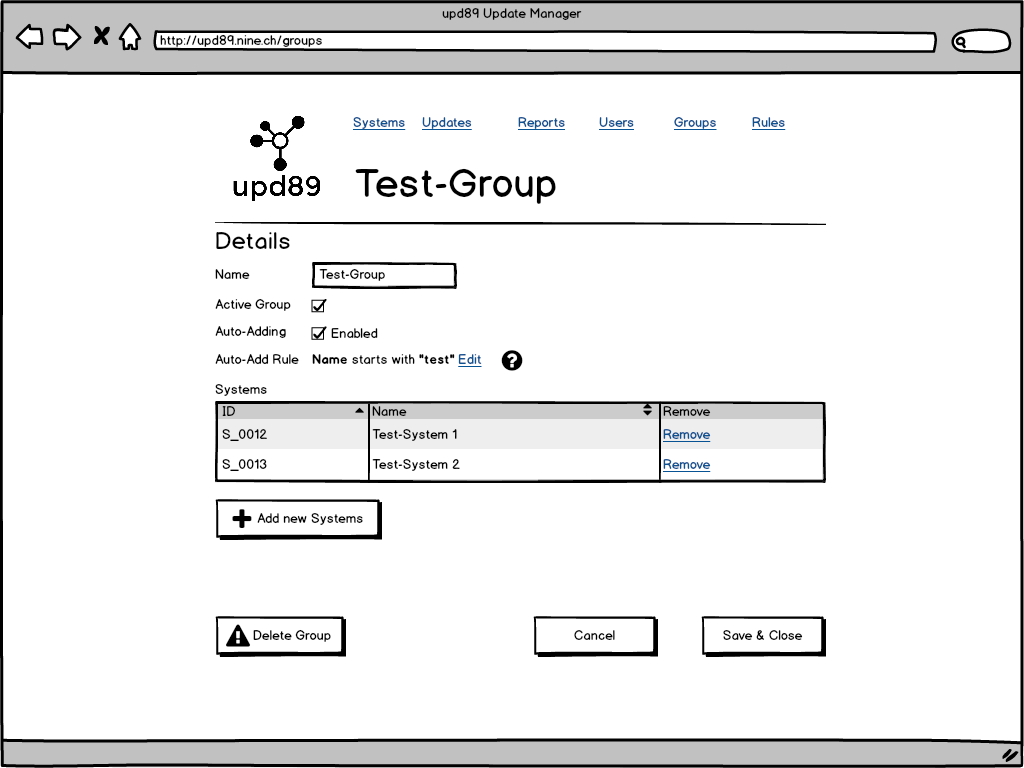
\includegraphics[width=\linewidth]{files/mockups/group_systems}
	\caption{Detail-Ansicht der System-Gruppe 'test-group'}
	\label{fig:design:group_systems_mockup}
\end{figure}

\subsubsection*{Berechtigungen}

Für den Use-Case 07 (siehe \ref{sec:uc_07}) wurden drei verschiedene Vorgehensweisen konzipiert. Die erste (Bild \ref{fig:design:permission_1}) sah vor, dass pro User die Einstellungen für jedes System, jede Art (Gruppe) von Anwendungen und sogar unterscheidend zwischen grossen oder kleinen Versionssprüngen vorgenommen werden kann. Dies wurde aber verworfen, da der Administrationsaufwand bei Änderungen zu gross gewesen wäre. Zudem kann nicht garantiert werden, dass 'grosse' Versionssprünge korrekt erkannt werden.

Eine Alternative sah weiterhin die Verwaltung der Rechte pro User vor, aber in einer tabellarischen Form mit simplen Ja/Nein-Berechtingen für verschiedene Aktionen (Bild \ref{fig:design:permission_2}). Hier wurde auch zwischen 'normalen' und 'kritischen' Updates unterschieden, also nur mit zwei Paketgruppen. Der Vorteil war die einfache Bedienung und die klare Darstellung der Berechtigungen. Aufgrund der gewünschten beliebigen Anzahl Paketgruppen wurde diese Alternative aber ebenfalls verworfen.

Schlussendlich hat sich eine Rollen- und stufenbasierte Rechteverwaltung durchgesetzt. Jeder Benutzer wird einer Rolle zugeteilt, welche eine bestimmte Berechtigungsstufe besitzt. Ob ein Benutzer nun ein Paket auf einem System aktualisieren darf, hängt von der benötigten Berechtigungsstufe der Gruppen des Paketes und des Systems ab.

Auf diese Weise ist es sehr einfach, ganzen Benutzergruppen die Rechte für mehrere Systeme oder Pakete auf einmal zu entziehen oder zu verteilen, was bei den alternativen Vorschlägen mindestens eine Einstellung pro User gewesen wäre.

\begin{figure}[H]
	\centering
	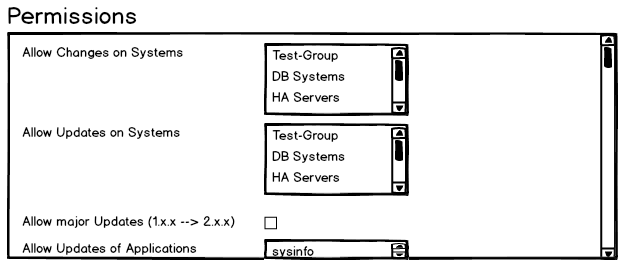
\includegraphics[width=0.75\linewidth]{files/mockups/permission_1}
	\caption{Rechtesystem}
	\label{fig:design:permission_1}
\end{figure}

\begin{figure}[H]
	\centering
	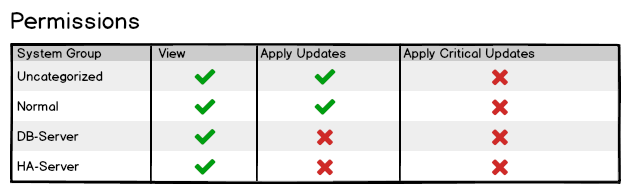
\includegraphics[width=0.75\linewidth]{files/mockups/permission_2}
	\caption{Rechtesystem (Alternative)}
	\label{fig:design:permission_2}
\end{figure}

\subsubsection*{Dashboard}

Eine Art Übersichtsseite war von Beginn an geplant und auch durch den Industriepartner begrüsst. Bei einer grösseren Anzahl von Systemen ist es oft einfacher, eine vereinfachte Zusammenfassung als eine detaillierte Auflistung aller einzelnen Systeme zu lesen. Dies und relevante Aktionen bei Auftreten von bestimmten Situationen anzubieten war das Ziel des Dashboards (Bild \ref{fig:design:dashboard_mockup}).

Einerseits sollte sichtbar sein, wieviele Systeme verfügbar sind, auf welchen Systemen Updates anstehen oder wo gerade Installationen durchgeführt werden. Andererseits sollten auch die letzten Aktivitäten und deren Ergebnis sichtbar sein, um schnell zu sehen, wo Probleme entstanden sind und wodurch diese ausgelöst worden sein könnten.

Da das Feature zur automatischen Zuweisung von neu registrierten Systemen und noch unbekannten Paketen in Gruppen verworfen wurde, musste dies nun manuell erledigt werden. Dazu wurde eine Auflisten dieser Systeme und Pakete auf dem Dashboard konzipiert, wo sie auch gleich in Gruppen eingeteilt werden konnten. 

\begin{figure}[H]
	\centering
	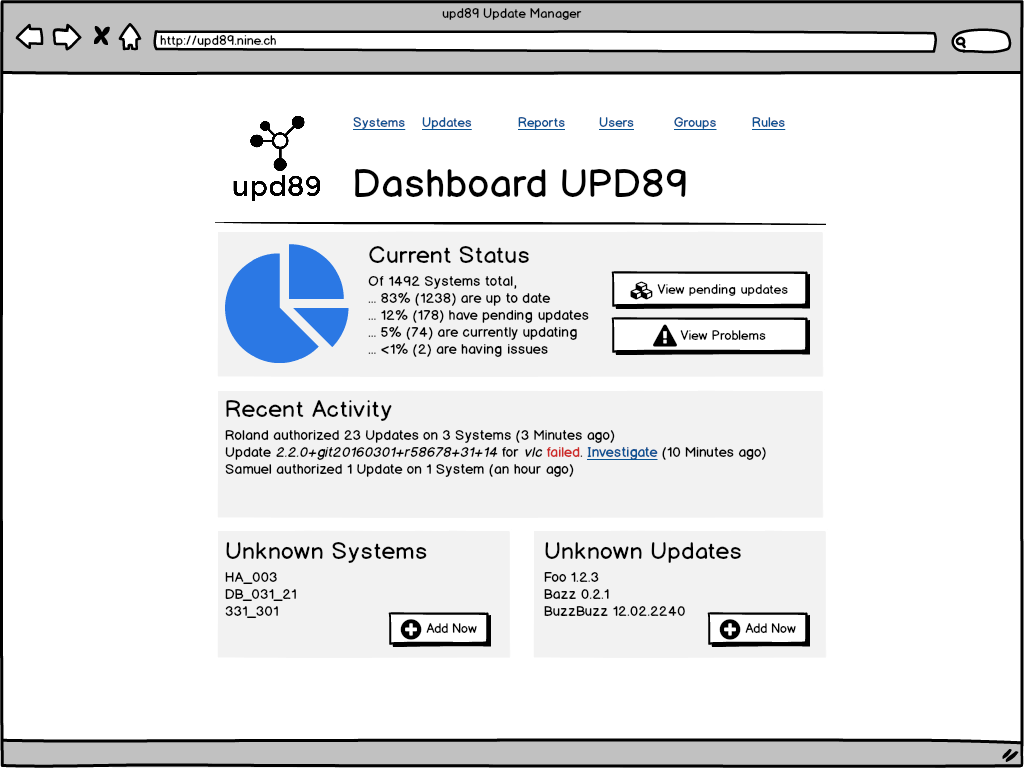
\includegraphics[width=\linewidth]{files/mockups/dashboard}
	\caption{Konzept des Dashboards}
	\label{fig:design:dashboard_mockup}
\end{figure}

\subsubsection*{System- und Paket-Ansicht}

Neben den spezifischen Ansichten für je alle Pakete oder Systeme mit entsprechenden Filtern, von wo aus Updatevorgänge gestartet werden können, war es ein Wunsch vom Industriepartner, auch eine kombinierte Ansicht zu haben, wo sowohl nach Paketen als auch nach Systemen gefiltert und gesucht werden kann. Nach mehreren Entwurfsiterationen wurde schliesslich Bild \ref{fig:design:combo_view_mockup} als passendes Design gefunden. Hier ist es möglich, mehrere Pakete gleichzeitig auf mehreren, einzeln aus- oder abwählbaren Systemen in Auftrag zu geben.

\begin{figure}[H]
	\centering
	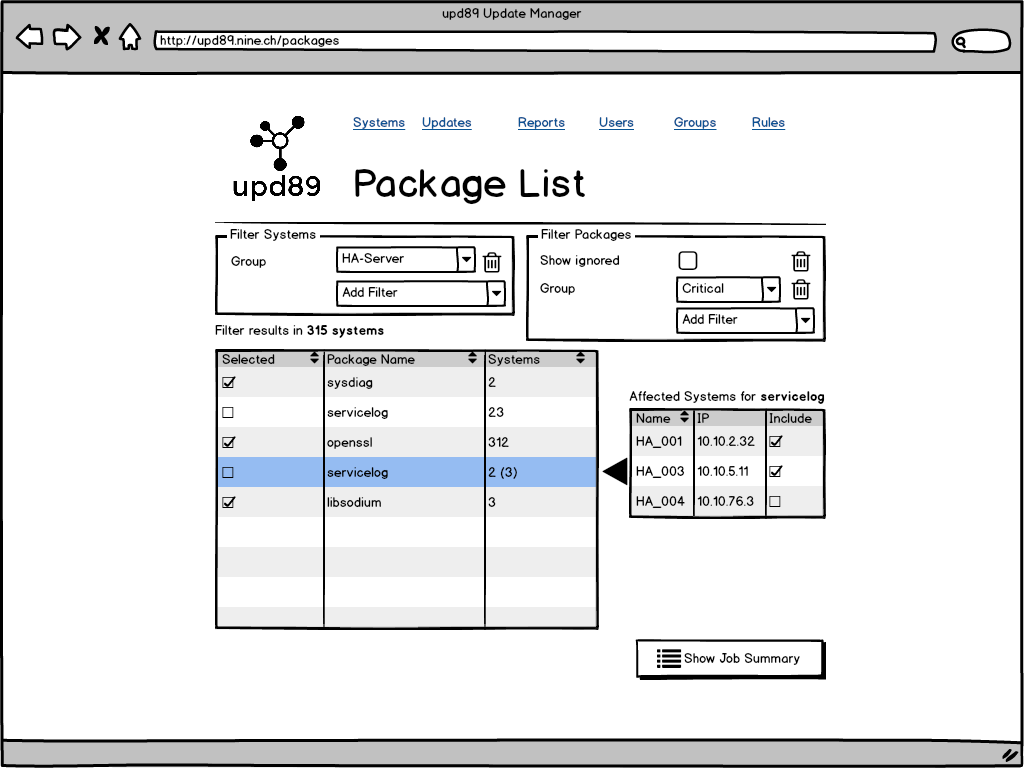
\includegraphics[width=\linewidth]{files/mockups/combo_view}
	\caption{Haupt-Ansicht mit Paket- und System-Filter}
	\label{fig:design:combo_view_mockup}
\end{figure}

\subsection*{User Interface}

Die Oberflächen halten sich mehrheitlich an die Mockups aus der Planung, einige Details wurden aber aufgrund von Input durch die Industriepartner oder durch 'Hallway-Testing'\footnote{Test mit zufällig ausgewählten Personen, ob ein Feature in der Benutzeroberfläche wie gedacht funktioniert.} abgeändert.

\begin{figure}[H]
	\centering
	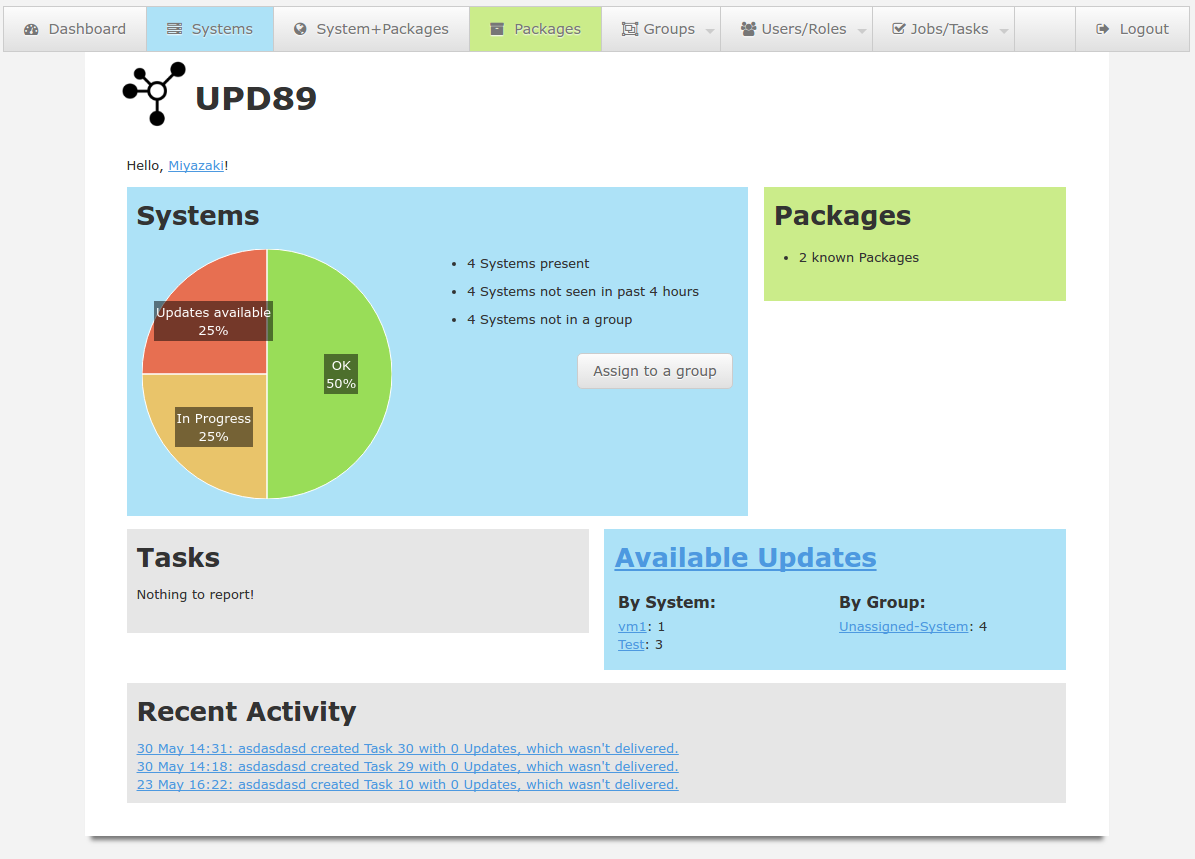
\includegraphics[width=\linewidth]{files/upd89-screenshot_dashboard}
	\caption{Umgesetztes Dashboard}
	\label{fig:design:dashboard}
\end{figure}

\subsection*{Logo, Icon, Schriftart}
Das Logo wurde in Squarespace Logo Generator\footnote{\purl{https://www.squarespace.com/logo/}} erstellt mit dem Icon 'Nodes'\footnote{\purl{https://thenounproject.com/search/?q=nodes+by+gregor&i=138240}} von Gregor Črešnar. Die Schriftart für 'UPD89' ist Montserrat\footnote{\purl{https://www.fontsquirrel.com/fonts/montserrat}} von Julieta Ulanovsky.

Das Icon wurde ge

\subsection*{Farben}

Generell wurde das Interface eher schlicht gehalten. Grautöne sowie Rot, Gelb und Grün als Signalfarben (\ref{fig:design:messages}) lassen die Seiten übersichtlich und nicht überladen erscheinen.

\begin{figure}[H]
	\centering
	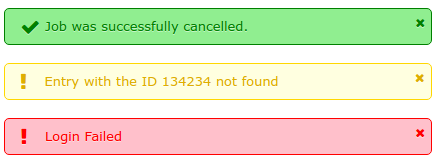
\includegraphics[width=0.5\linewidth]{files/messages}
	\caption{Beispiele der drei Hinweise 'Erfolg', 'Warnung', 'Error'}
	\label{fig:design:messages}
\end{figure}

Die selbst definierten Farben wurden in einer separaten \gls{scss}-Datei definiert, wodurch es für anwendungs- oder benutzerspezifische Anpassungen einfach abzuändern ist. Eine Übersicht über die wichtigsten Farben ist in Bild \ref{fig:design:colorcodes} zu sehen.

\begin{figure}[H]
	\centering
	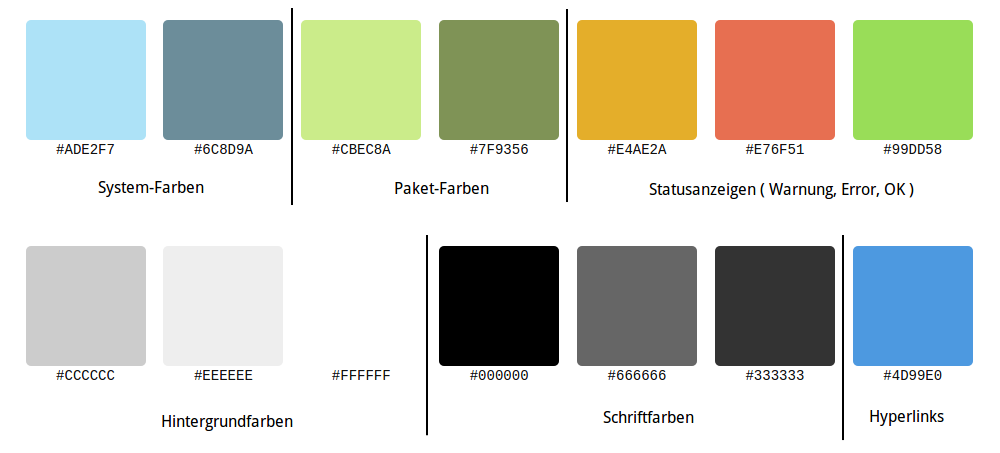
\includegraphics[width=\linewidth]{files/colorcodes}
	\caption{Verwendete Farben mit Hex-Codes}
	\label{fig:design:colorcodes}
\end{figure}

Ein besonderes Augenmerk wurde auf die farbliche Kennzeichnung der Systeme und Pakete gelegt. Besonders in der kombinierten Ansicht, wo es Filtermöglichkeiten zu Systemen und zu Paketen gibt, ist es mit einer farblichen Unterscheidung einfacher zu sehen, was welche Entitätsgruppe betrifft. Diese Farben wurden auch ins Menu und ins Dashboard weitergezogen; in der ganzen Applikation sind Infos und Einstellungen, welche zu Systemen relevant sind, generell im 'System-Blau', solche für Pakete im 'Paket-Grün' (Beispiel im Bild \ref{fig:design:sys_pkg_colors}).

\xxx[ref zu combo-view?]

\begin{figure}[H]
	\centering
	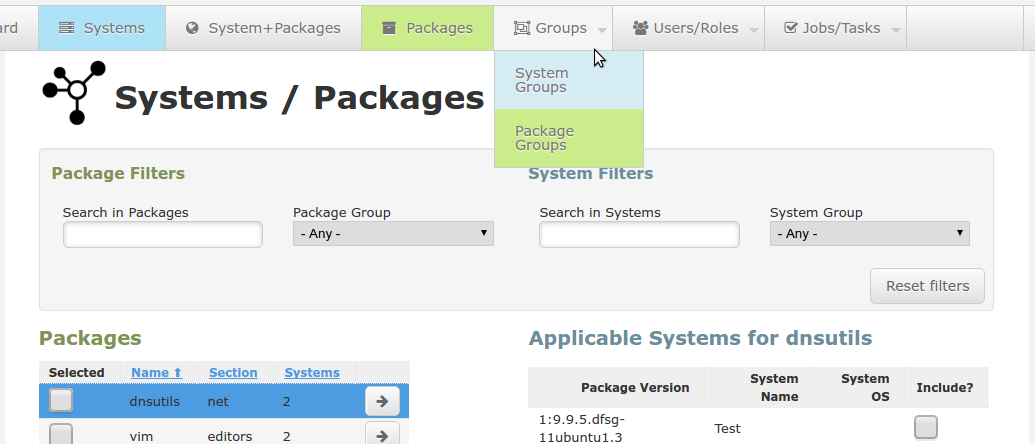
\includegraphics[width=\linewidth]{files/colors_pkg_sys}
	\caption{Simple Farb-Hinweise: Blau für Systeme, Grünlich für Pakete}
	\label{fig:design:sys_pkg_colors}
\end{figure}

\subsubsection*{Building Blocks}

Um verschiedene grafische Elemente konsistent gleich aussehen zu lassen, wurde das HTML Kickstart-Framework von Joshua Gatcke/99lime.com\footnote{\purl{http://www.99lime.com/elements/}} verwendet. Dadurch waren gewisse Funktionalitäten wie etwa das Menu oder die Hinweise bereits vorhanden.


Für die Icons wurde FontAwesome\footnote{\purl{http://fontawesome.io/}} verwendet.
